% !TEX TS-program = pdflatex
% !TEX encoding = UTF-8 Unicode


\documentclass[12pt,a4paper]{article}

\usepackage[french]{babel}
\usepackage[T1]{fontenc}
\usepackage[utf8]{inputenc}

\usepackage{amsmath,amsfonts,amssymb}

\usepackage{geometry}
\geometry{margin=75pt}

\usepackage[upright]{fourier}
\usepackage{subfig}

\usepackage{shadethm}

\usepackage{color}
\definecolor{gris_clair}{gray}{.9}
\definecolor{gris}{gray}{.35}
\definecolor{vert}{rgb}{0,0.5,0}
\definecolor{rouge}{rgb}{0.5,0,0}
\definecolor{turquoise}{rgb}{0,0.5,0.5}

\usepackage{listings}
\usepackage{paralist}
\usepackage{stmaryrd}
\usepackage{tikz}
\usetikzlibrary{shapes.multipart}
\usetikzlibrary{calc}

\lstset{
language=Python,
backgroundcolor=\color{gris_clair},
frame=single,
basicstyle=\footnotesize\ttfamily\color{gris},
identifierstyle=\color{black},
keywordstyle=\color{vert},
stringstyle=\color{rouge}, showstringspaces=false,
commentstyle=\itshape\color{turquoise},
%numbers=left, numbersep=5pt, numberstyle=\color{gris}\tiny,stepnumber=5,
breaklines=true,
literate=
  {é}{{\'e}}1 {É}{{\'E}}1 {à}{{\`a}}1 {è}{{\`e}}1% 
  {À}{{\`A}}1 {È}{{\'E}}1 {ë}{{\"e}}1 {ï}{{\"i}}1%
  {â}{{\^a}}1 {ê}{{\^e}}1 {î}{{\^i}}1 {ô}{{\^o}}1% 
  {û}{{\^u}}1 {Â}{{\^A}}1 {Ê}{{\^E}}1 {Î}{{\^I}}1%
  {Ô}{{\^O}}1 {œ}{{\oe}}1 {Œ}{{\OE}}1 {æ}{{\ae}}1%
  {Æ}{{\AE}}1 {ç}{{\c c}}1 {Ç}{{\c C}}1 {€}{{\EUR}}1 ,
morekeywords={len,input,range}}         


\title{Comment optimiser l'architecture d'un réseau pour résister aux attaques ?\\ \bigskip
  Rapport final de TIPE}
%
% Propagation des informations dans un réseau pair-à-pair
%
%

\author{Matthias Goffette}
\date{}

\begin{document}
\maketitle

%\section*{Abstract} % 100 words | 78 words

%Networks need to be reliable, so that they can resist accidents and attacks.
%We focus on two types of networks: homogenous and scale-free.
%We model networks as graphs and perform agent-based simulations.
%On these, attacks are performed : attackers falsify the information before spreading it.
%The simulations show that for the same mean degree of nodes, homogenous networks are less resiliant than scale-free networks.
%In scale-free networks, resistance depends on sum of degrees of attackers.



\section{Préambule} % 75 mots | 70 mots

Mon objectif a peu changé depuis la MCOT.
J'ai poursuivi l'étude de l'impact d'une attaque sur les noeuds du réseau selon sa topologie.
C'est là que réside la différence avec le travail de Dimitri Granger, l'autre membre du groupe, qui s'est intéressé à des attaques sur les liens.
Je ne me suis finalement pas concentré sur la vitesse de transmission des informations car cette partie m'a semblé moins intéressante.


\section{Introduction} % 100 mots | 96 mots
% Le  candidat  doit  introduire  de  façon  claire  et  synthétique  le travail  qu’il  a effectivement réalisé, en cohérence avec son préambule.


Sécuriser les réseaux informatiques est aujourd'hui un point primordial.
En effet, ils sont le support de communications de plus en plus nombreuses entre les ordinateurs.
Dans ce cadre, je me suis intéressé à l'effet de l'architecture d'un réseau sur sa vulnérabilité aux attaques.
Pour apporter des éléments de réponse à cette question, j'ai utilisé une modélisation multi-agents en langage Python.
J'ai effectué des simulations sur deux types de réseaux, \emph{scale-free} et \emph{homogène}.
J'ai fait varier deux paramètres de la taille du réseau : le nombre de nœuds et le nombre d'arêtes par nœud.  


\section{Corps Principal} %750 mots | 411 mots

\subsection{Modalités d'action} % 250 | 220 mots

Il a fallu tout d'abord définir la manière dont une attaque allait opérer.
Un noeud peut être soit normal, soit attaquant.
Un noeud normal transmettra à ses voisins les informations qu'il reçoit sans les modifier.
Mais un attaquant, avant de transmettre des informations, les faussera.

J'ai ensuite choisi la représentation des objets utiles pour la modélisation.
J'ai utilisé des objets Pythons : les agents qui représentent les noeuds du réseau, les tunnels qui représentent les arêtes, et un objet qui rassemble les deux premiers, le réseau.
Un dernier objet, l'information, est utilisé pour observer la propagation d'informations faussées par les attaquants.
Une information peut prendre deux valeurs, vrai ou faux.

J'ai généré des réseaux \emph{scale-free} avec l'algorithme de Barabási–Albert.
Il consiste à prendre un graphe initial, et à ajouter des nœuds.
A chaque ajout d'un nœud $i$, on le lie à un nœud $j$ avec une probabilité proportionnelle au degré de $j$.
Cela crée un réseau dans lequel la probabilité qu'un nœud ait $k$ voisins est $\alpha k^{-\gamma}$.
Ici, $\gamma = 3$ et $\alpha \approx 0.83$.
Ainsi, quelques nœuds ont une forte connectivité, et une majorité en ont une faible.
Pour générer des réseaux homogènes, j'ai utilisé la bibliothèque Python NetworkX.

J'ai défini le plan d'expériences et conçu l'architecture du code me permettant de le réaliser.

Dans le cas des réseaux homogènes, j'ai considéré des réseaux ayant 10, 50 puis 100 nœuds, avec dans chaque cas trois arêtes par nœud.
J'ai également fait varier le nombre d'arêtes par nœud, pour un réseau de 50 agents, avec des degrés de 3 et 20 successivement.

Pour chaque jeu de paramètres, j'ai effectué 100 simulations.
Une simulation consiste en la génération d'un réseau.
Pour chacun de ces réseaux, le nombre d'attaquants varie entre 0 et le nombre de nœuds $n$ du réseau.
Pour chacun de ces cas, l'algorithme effectue une diffusion de l'information dans le réseau.
Il en résulte une proportion d'informations fausses en fonction du nombre d'attaquants.
La comparaison de la vulnérabilité des différents réseaux en fonction de leur architecture se fonde sur la moyenne des 100 simulations. 

\subsection{Restitution des résultats} %300 | 303


Sur les réseaux homogènes, j'observe que le nombre d'informations fausses dans le réseau croît avec le nombre d'attaquants (figure~\ref{noeuds}).
La courbe est concave : plus il y a d’attaquants, moins l’action d’en ajouter un nouveau a un effet important.
Cela s'explique par une redondance d'informations fausses.

\begin{center}
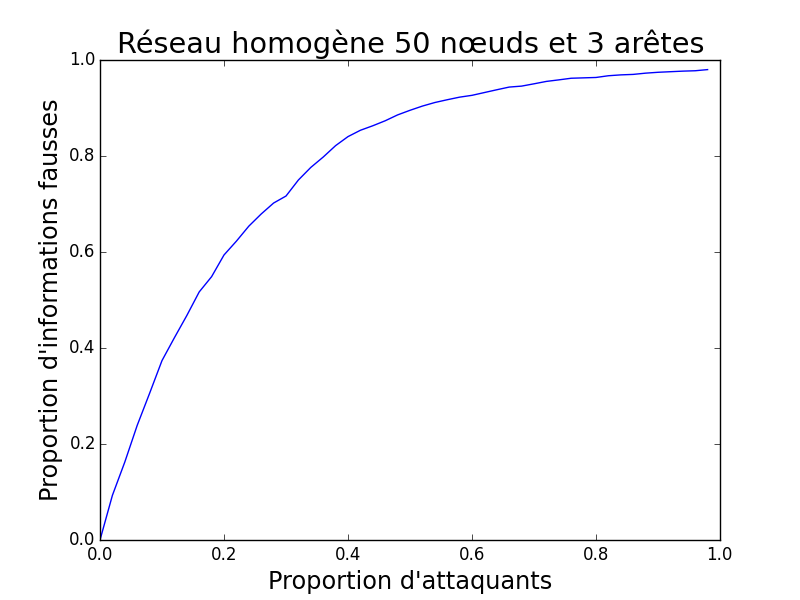
\includegraphics[width=0.49\linewidth]{../resultats/atkaleat/atkaleat-50-3-2-i100.png}
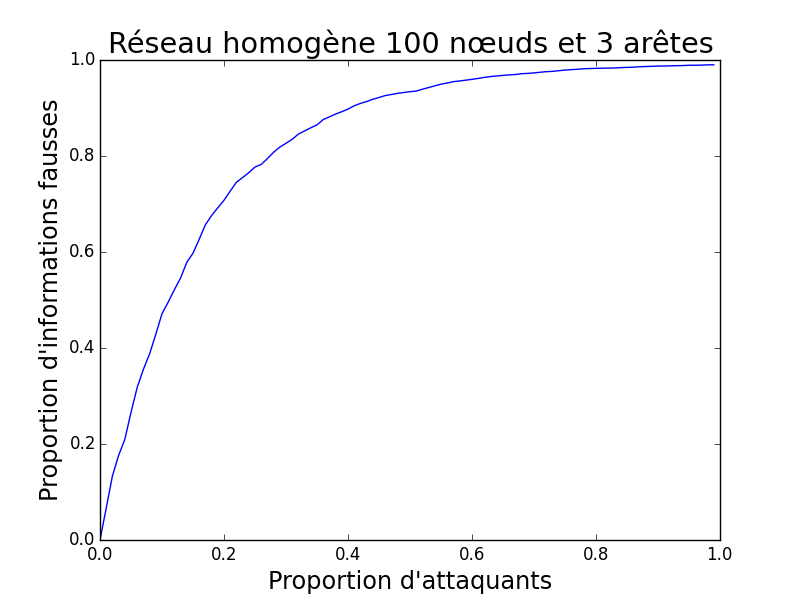
\includegraphics[width=0.49\linewidth]{../resultats/atkaleat/atkaleat-100-3-1-i100.png}
\captionof{figure}{Réseau homogène - Variation du nombre de nœuds} \label{noeuds}
\end{center}

Pour un nombre de nœuds constant, l'augmentation du nombre d'arêtes par nœuds se traduit, au-delà d'un certain seuil, par l'apparition d'une partie affine de la courbe, qui correspond à un stade où les seuls nœuds non attaquants sont voisins de l'émetteur (figure~\ref{aretes}).

\begin{center}
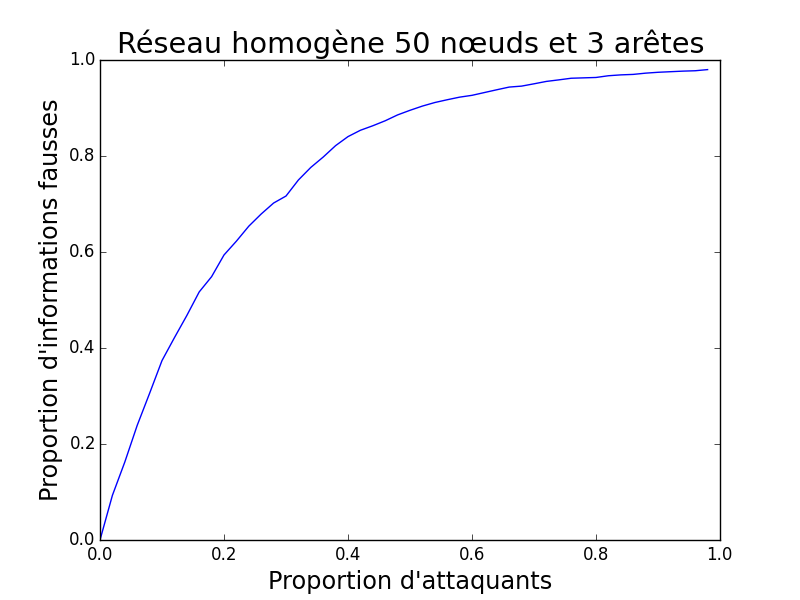
\includegraphics[width=0.49\linewidth]{../resultats/atkaleat/atkaleat-50-3-2-i100.png}
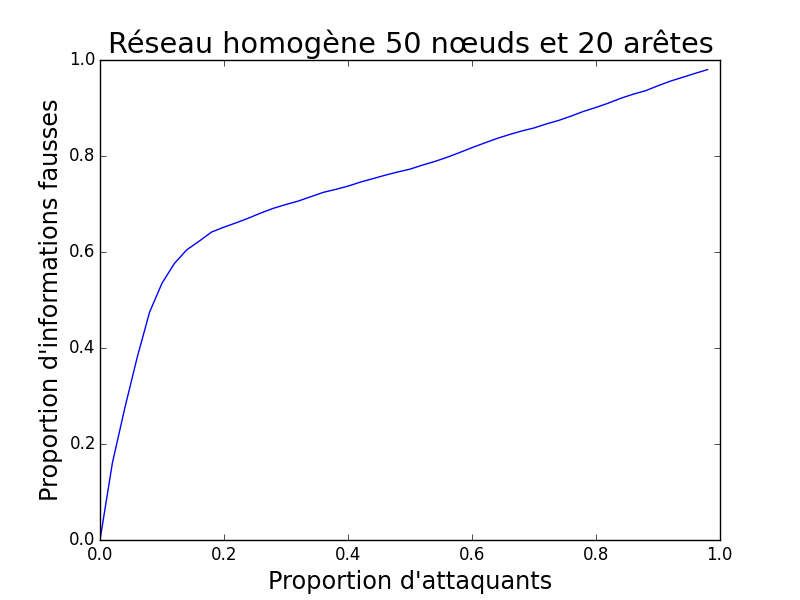
\includegraphics[width=0.49\linewidth]{../resultats/atkaleat/atkaleat-50-20-2-i100.png}
\captionof{figure}{Réseau homogène - Variation du nombre d'arêtes par nœud} \label{aretes}
\end{center}

Dans le cas des réseaux invariants d'échelle, on observe en moyenne le même type de courbe concave que pour un réseau homogène.
Cependant, pour une simulation donnée, la courbe présente des paliers (figure \ref{sf}).
Lorsqu'un nœud ayant une forte connectivité devient attaquant, il a un fort impact sur le reste du réseau.

Pour une même somme de degrés des nœuds attaquants, le nombre d'attaquants est très variable (figure \ref{deg}).
Or, la somme des degrés des nœuds attaquants est une mesure de l'influence des attaquants.
Sur certains réseaux, les nœuds ayant des degrés élevés seront contaminés assez tôt, alors que sur d'autres, ils seront contaminés au contraire assez tardivement.


\begin{center}
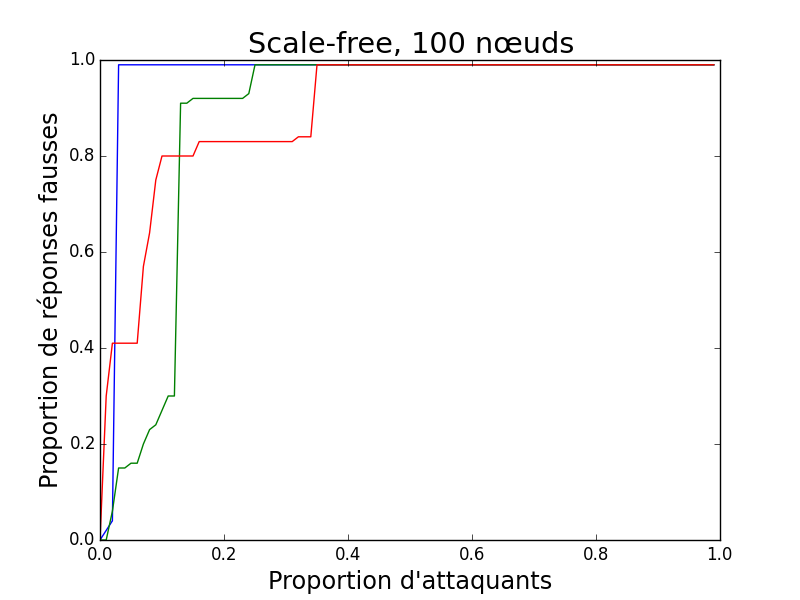
\includegraphics[width=0.49\linewidth]{../resultats/scale-free/sf-t1s-n100-2-it3.png}
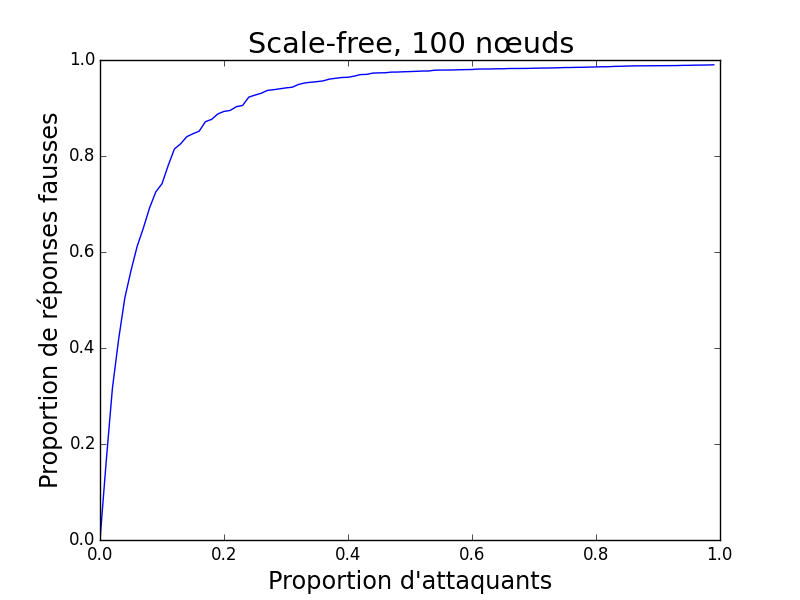
\includegraphics[width=0.49\linewidth]{../resultats/scale-free/sf-t1-n100-1-it100.png}
\captionof{figure}{Réseaux scale-free - Courbes de trois simulations et moyenne sur cent simulations} \label{sf}
\end{center}

\begin{center}
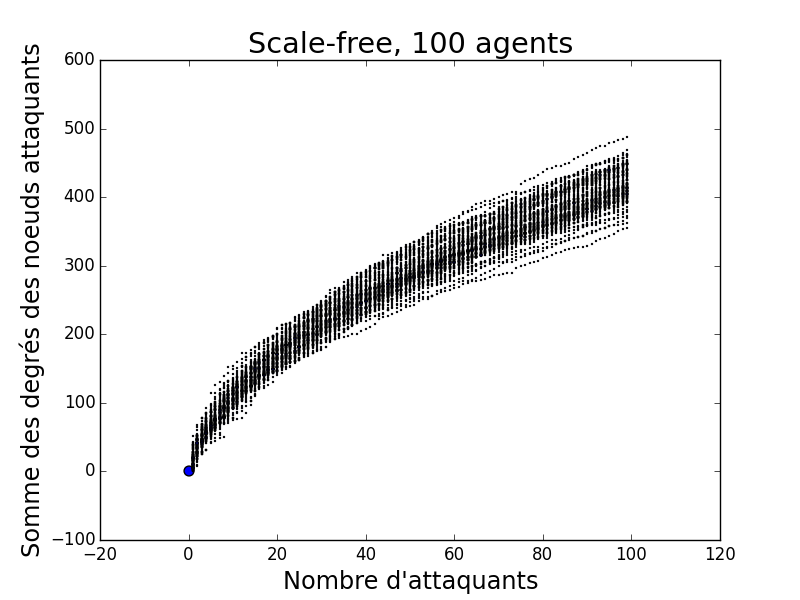
\includegraphics[width=0.49\linewidth]{../resultats/scale-free/sf-t2-n-100-1-it100.png}
\captionof{figure}{Somme des degrés attaquants selon le nombre d'attaquants} \label{deg}
\end{center}

Pour comparer les réseaux scale-free et homogènes, j'ai généré plusieurs réseaux invariants d'échelle ayant 100 nœuds et calculé le degré moyen par nœud, grâce à un script Python.
Le degré moyen vaut deux pour un réseau généré avec l'algorithme de Barabási–Albert.
Or, on constate que les réseaux homogènes de degré deux ont en moyenne une plus grande proportion d'informations fausses (voir figure \ref{comp}).


\begin{center}
  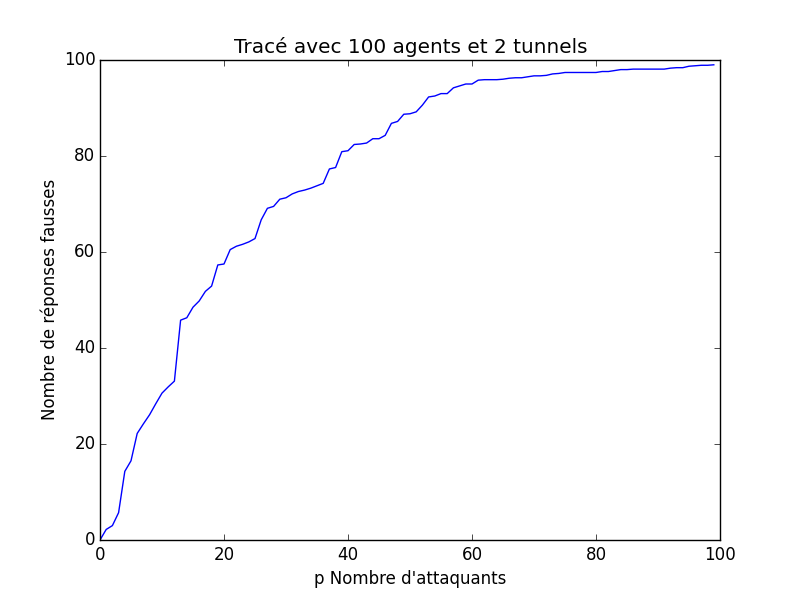
\includegraphics[width=0.49\linewidth]{../resultats/atkaleat/atkaleat-100-2-1.png}
  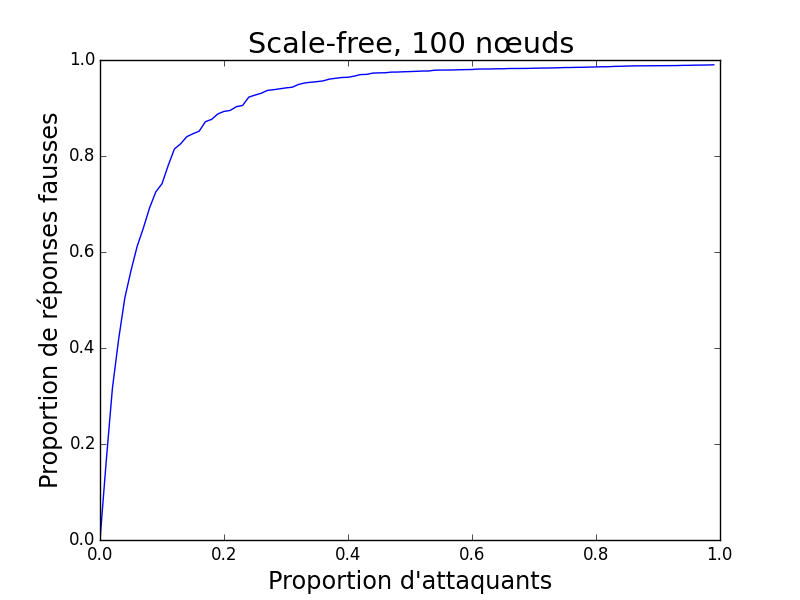
\includegraphics[width=0.49\linewidth]{../resultats/scale-free/sf-t1-n100-1-it100.png}
  \captionof{figure}{Comparaison des réseaux homogène et invariant d'échelle} \label{comp}
\end{center}
	



\subsection{Analyse - Exploitation - Discussion} %200 | 217

Pour les réseaux homogènes et invariants d'échelle, l'attaque modélisée contamine le réseau très rapidement.
D'après mes simulations, il suffit de 20\% d'attaquants pour contaminer plus de la moitié du réseau.
De plus, l'augmentation du nombre de nœuds dans un réseau homogène ne va pas diluer les informations fausses, mais au contraire renforcer l'effet des attaquants.
On peut appréhender ce phénomène en considérant que les modélisations effectuées sont équivalentes à créer un arbre dont la racine est le nœud responsable de l'émission de l'information, et dont les branches sont les chemins suivis par l'information.
Ajouter des nœuds revient à augmenter la taille de l'arbre.
Les nœuds attaquants sont distribués dans tout l'arbre, mais plus ils sont près de la racine, plus ils ont d'influence.

Les résultats sur les réseaux homogènes peuvent être intéressants, notamment dans le cas où chaque nœud à un degré élevé.
Mais ce type de réseau est peu facile à mettre en pratique.
C'est donc un objet principalement théorique.

Une limite du modèle concerne la probabilité pour un nœud d'être attaquant.
Je l'ai considérée comme uniforme, or en pratique, les serveurs très connectés sont de gros serveurs, généralement plus protégés que les autres.
Ils devraient donc être moins souvent infectés, ce qui augmente les performance des réseaux invariants d'échelle.



\section{Conclusion générale} %75 mots | 74 mots

Les réseaux homogènes semblent être moins robustes que les réseaux invariants d'échelle.
Cependant, augmenter le degré moyen des réseaux homogènes permet d'accroître leur résistance aux attaques.

L'étude de l'autre membre du groupe considère des attaques sur les arêtes pour des graphes de Harary et en étoile.
L'architecture optimale dépend alors du coût de protection.

Les réseaux scale-free sont des groupements de réseaux en étoile, et les réseaux de Harary sont des réseaux homogènes.

% scale-free <-> étoile
% homogène <-> Harary
% si faible coût de protection, étoile > Harary
% si élevé, Harary > étoile
% Or dans ce que je fais, pas de coût de protection, et sf (qui est une fédération d'étoiles) > homogène
% par contre, si protection non uniforme, sf > homogène

\end{document}
%\grid
